% https://www.sharelatex.com/blog/2013/08/27/tikz-series-pt1.html

\documentclass[tikz]{standalone}
\usetikzlibrary{patterns}
\begin{document}
\newcommand{\drawstencil}[2]{%
  \draw[darkgray, thick, pattern=north west lines, pattern color=gray] (#1-1, #2) rectangle (#1+2, #2+1);
  \draw[darkgray, thick, pattern=north west lines, pattern color=gray] (#1, #2-1) rectangle (#1+1, #2+2);
  \draw[darkgray, thick, pattern=north east lines, pattern color=gray](#1, #2) rectangle (#1+1, #2+1);
}
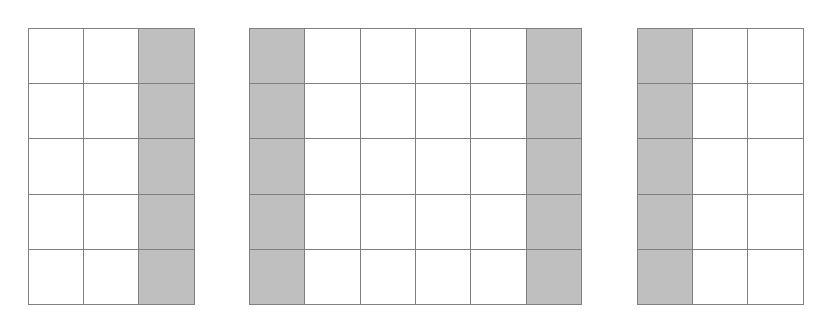
\begin{tikzpicture}[x=2em,y=2em]

  \fill[lightgray](-2,0) rectangle (-1, 5);
  \fill[lightgray] (0,0) rectangle (1,5);
  \fill[lightgray] (5,0) rectangle (6,5);
  \fill[lightgray](7,0) rectangle (8, 5);


  \draw[step=1, gray, very thin] (-4,0) grid (-1, 5);
  \draw[step=1, gray, very thin] (0,0) grid (6, 5);
  \draw[step=1, gray, very thin] (7,0) grid (10, 5);


  \drawstencil{2}{2}

\end{tikzpicture}
\end{document}
